\section{Aplicação: Dinâmica de Formas}\label{secao:simulacao_dinamica_de_formas}

Na seção \ref{secao:dinamica_de_formas} apresentamos uma breve introdução à Dinâmica de Formas sobre o PNCG, onde introduzimos a \textit{complexidade} $C_S$ como uma medida de evolução de um sistema e também as \textit{coordenadas objetivas} $(\vet \sigma, \vet \pi)$ sobre o espaço de formas. Nesta seção, visualizaremos alguns dos resultados apresentados.

Todas as simulações utilizadas aqui foram feitas com momento angular total $\vet J = \vet 0$, momento linear total $\vet P = \vet 0$ e centro de massas $\vet q_{cm} = \vet 0$. A energia foi testada com diferentes valores para diferentes objetivos, e os valores são explicitados em cada caso.



%%%%%%%% PROBLEMAS DE 3 CORPOS
\subsection{Problemas de 3 corpos}

Para visualizar as coordenadas objetivas $(\vet \sigma, \vet \pi)$, tomamos primeiramente um problema de 3 corpos com uma trajetória simples: um par kepleriano e um corpo ejetado, como na figura \ref{fig:probmodel_3_corpos_energia0_trajetoria}. Trata-se do problema-modelo \ref{probmodelo:3corpos_energia_nula}, integrado no intervalo $[0,50]$ via método de Verlet com $h=10^{-3}$, sem correção.

Este é um sistema com energia total 0, então os resultados da Dinâmica de Formas se aplicam. Por exemplo, a ejeção de um dos corpos corresponde a um atrito no espaço de fases (tomando a coordenada $\vet \omega$). Além disso, a complexidade (figura \ref{fig:3corpos_energia0_complexidade}) aumenta no sentido futuro devido à separação do sistema em dois, embora possua fortes oscilações ligadas às aproximações do sistema binário.

\begin{figure}[H]
    \centering
    
    \begin{subfigure}{.5\textwidth}
        \centering
        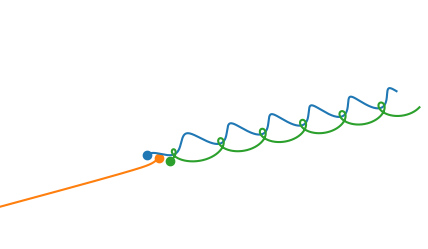
\includegraphics[width=0.8\linewidth]{tcc/img/sd/3corpos_energia0_posicoes_nd_2.png}
        \caption{}
        \label{fig:probmodel_3_corpos_energia0_trajetoria}
    \end{subfigure}%
    \begin{subfigure}{.5\textwidth}
        \centering
        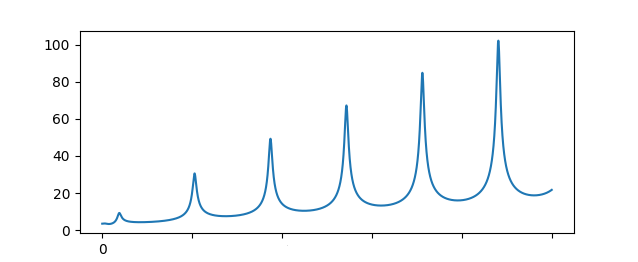
\includegraphics[width=\linewidth]{tcc/img/sd/3corpos_energia0_complexidade.png}
        \caption{}
        \label{fig:3corpos_energia0_complexidade}
    \end{subfigure}

    \caption{Problema-modelo \ref{probmodelo:3corpos_energia_nula}. À esquerda, recorte das trajetórias. À direita, a complexidade apresentada pelo sistema.}
    \label{fig:figuras_probmodel_3_energia0}
\end{figure}

Na figura \ref{fig:3corpos_energia0_posicoes_sd} é possível observar os comportamentos de ejeção e de formação de binários. Embora o corpo ejetado se afaste a princípio, conforme o par binário se forma, o ejetado desacelera e inicia uma trajetória cíclica e dissipativa. E, de fato, conforme a figura \ref{fig:3corpos_energia0_velocidades_sd} mostra, o corpo ejetado está desacelerando, enquanto o momento de forma ($\vet \pi$) dos outros dois apresenta trajetórias circulares com um raio cada vez maior e cada vez mais rapidamente. 

\begin{figure}[H]
    \centering
    \begin{subfigure}{.5\textwidth}
        \centering
        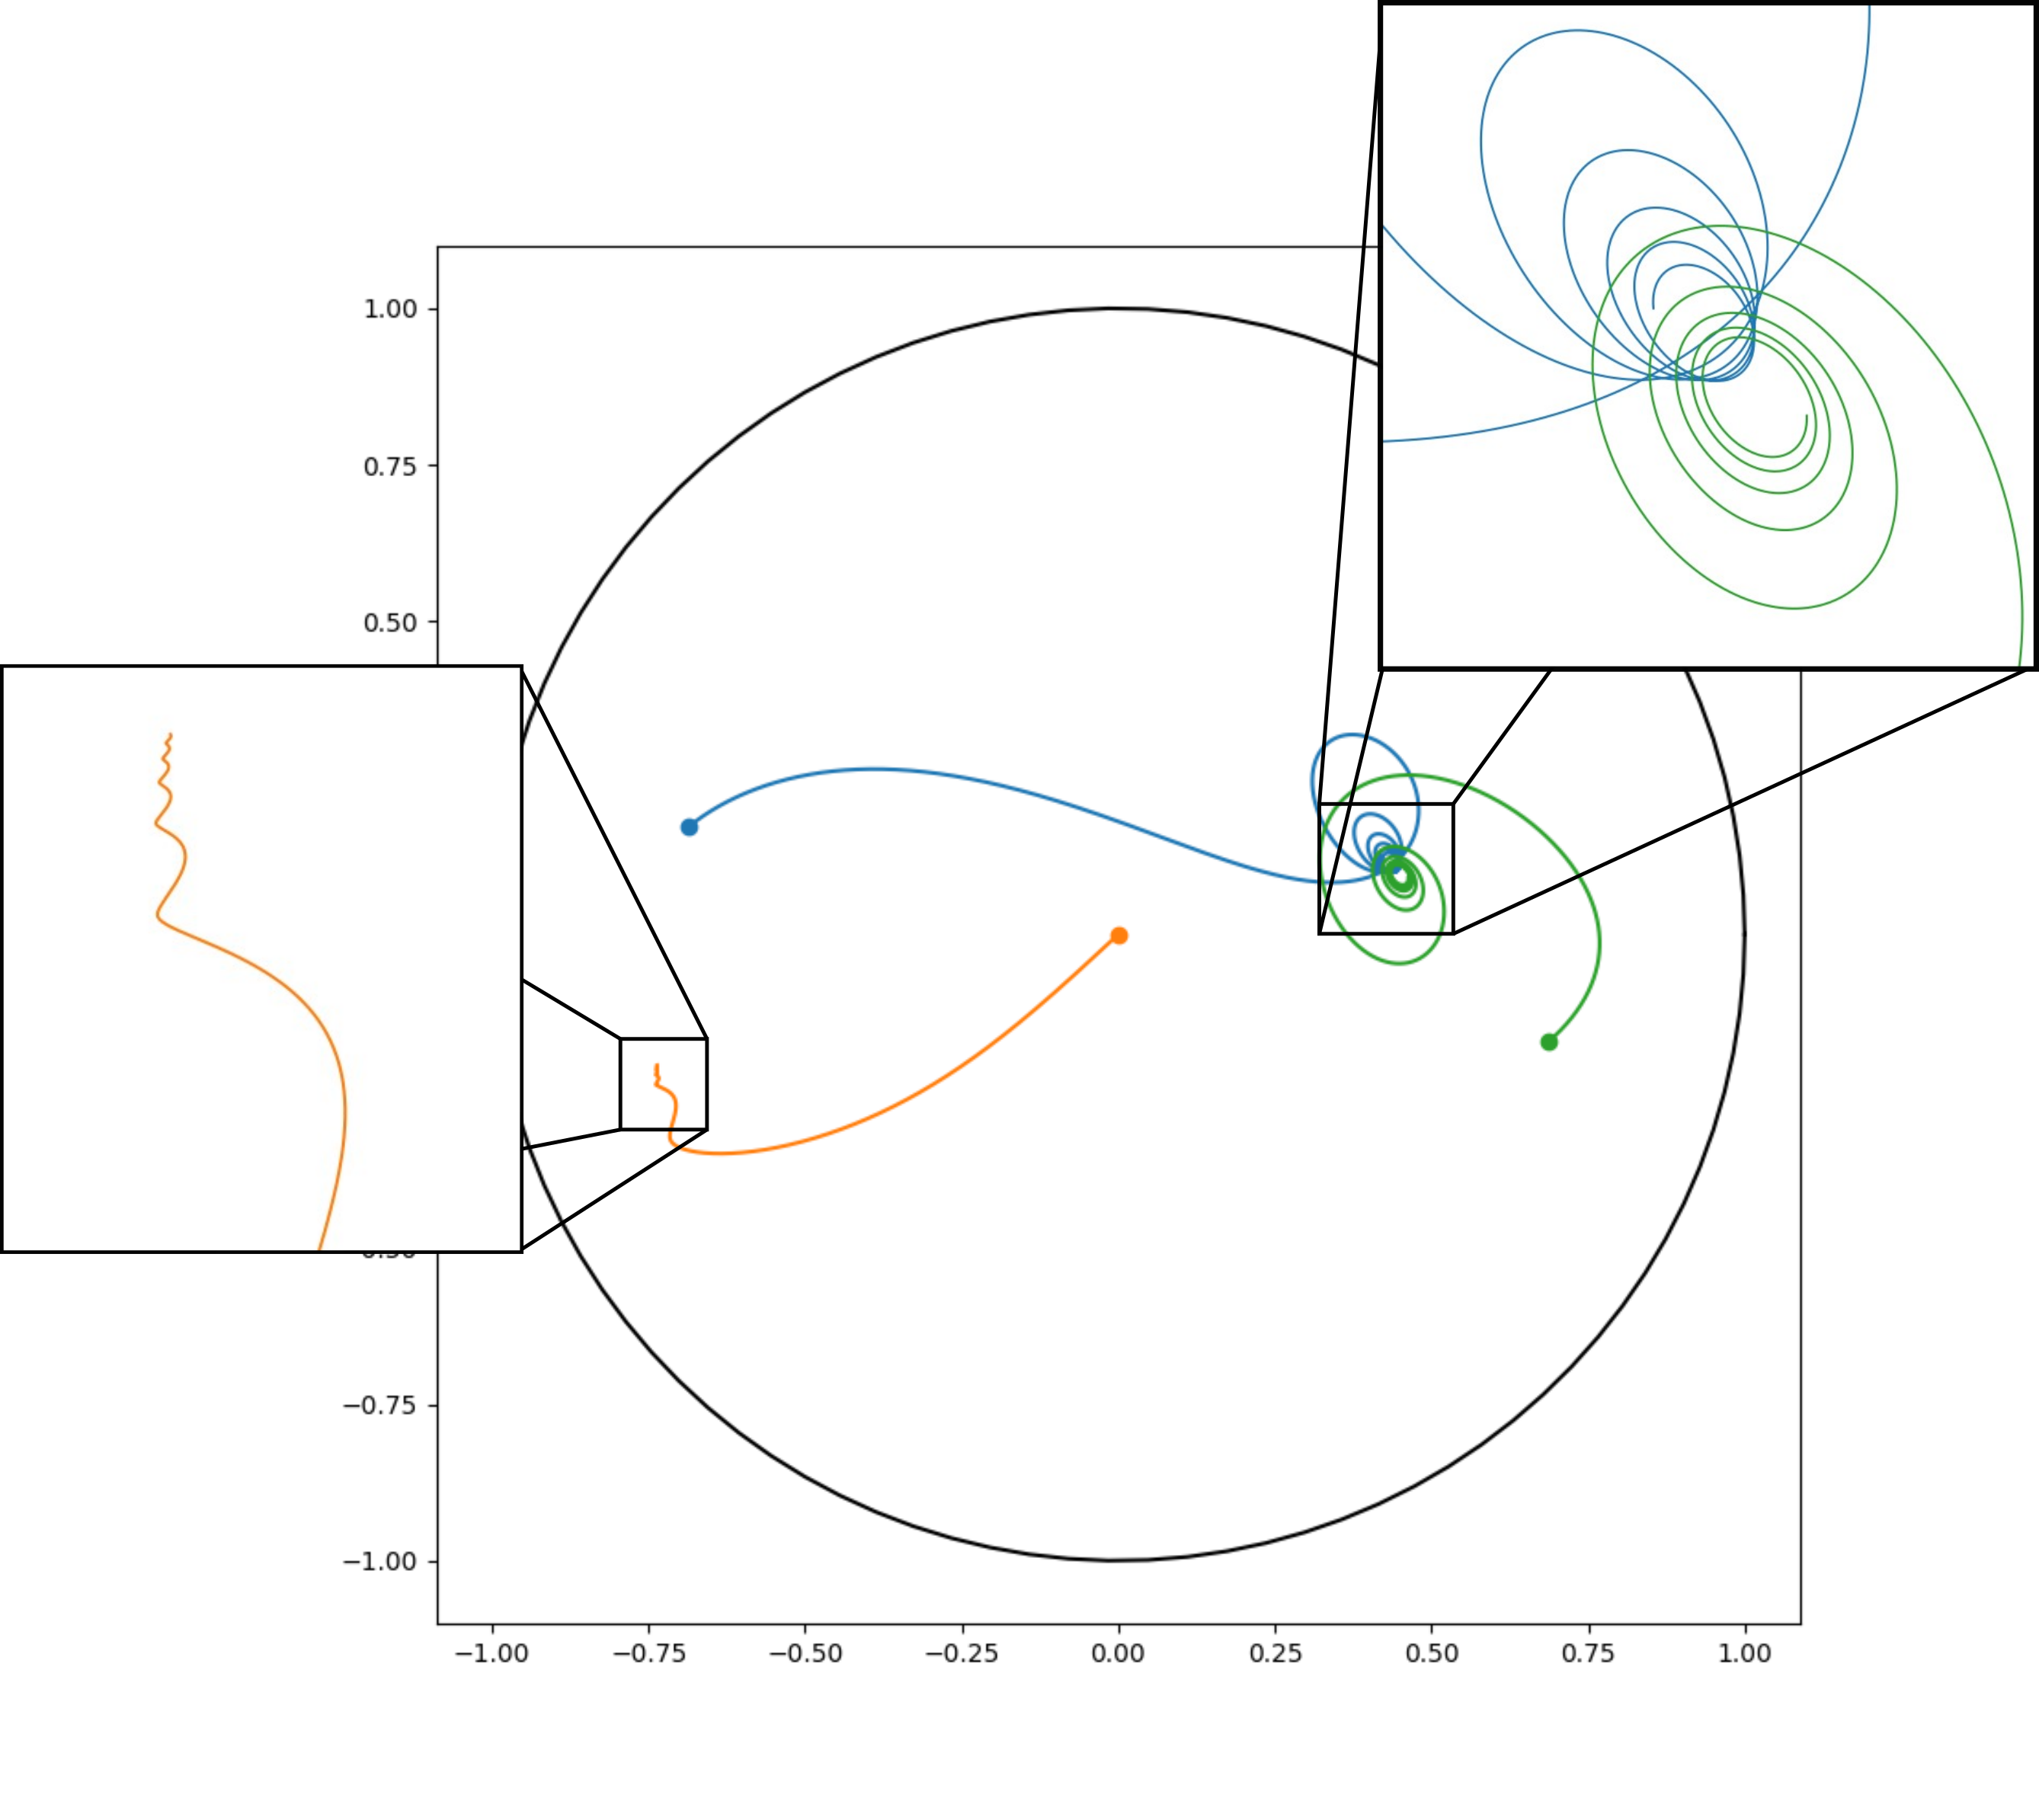
\includegraphics[width=\linewidth]{tcc//img/3corpos_energia0_posicoes_sd_zoom.png}
        \caption{Coordenadas de forma ($\vet \sigma$).}
        \label{fig:3corpos_energia0_posicoes_sd}
    \end{subfigure}%
    \begin{subfigure}{.5\textwidth}
        \centering
        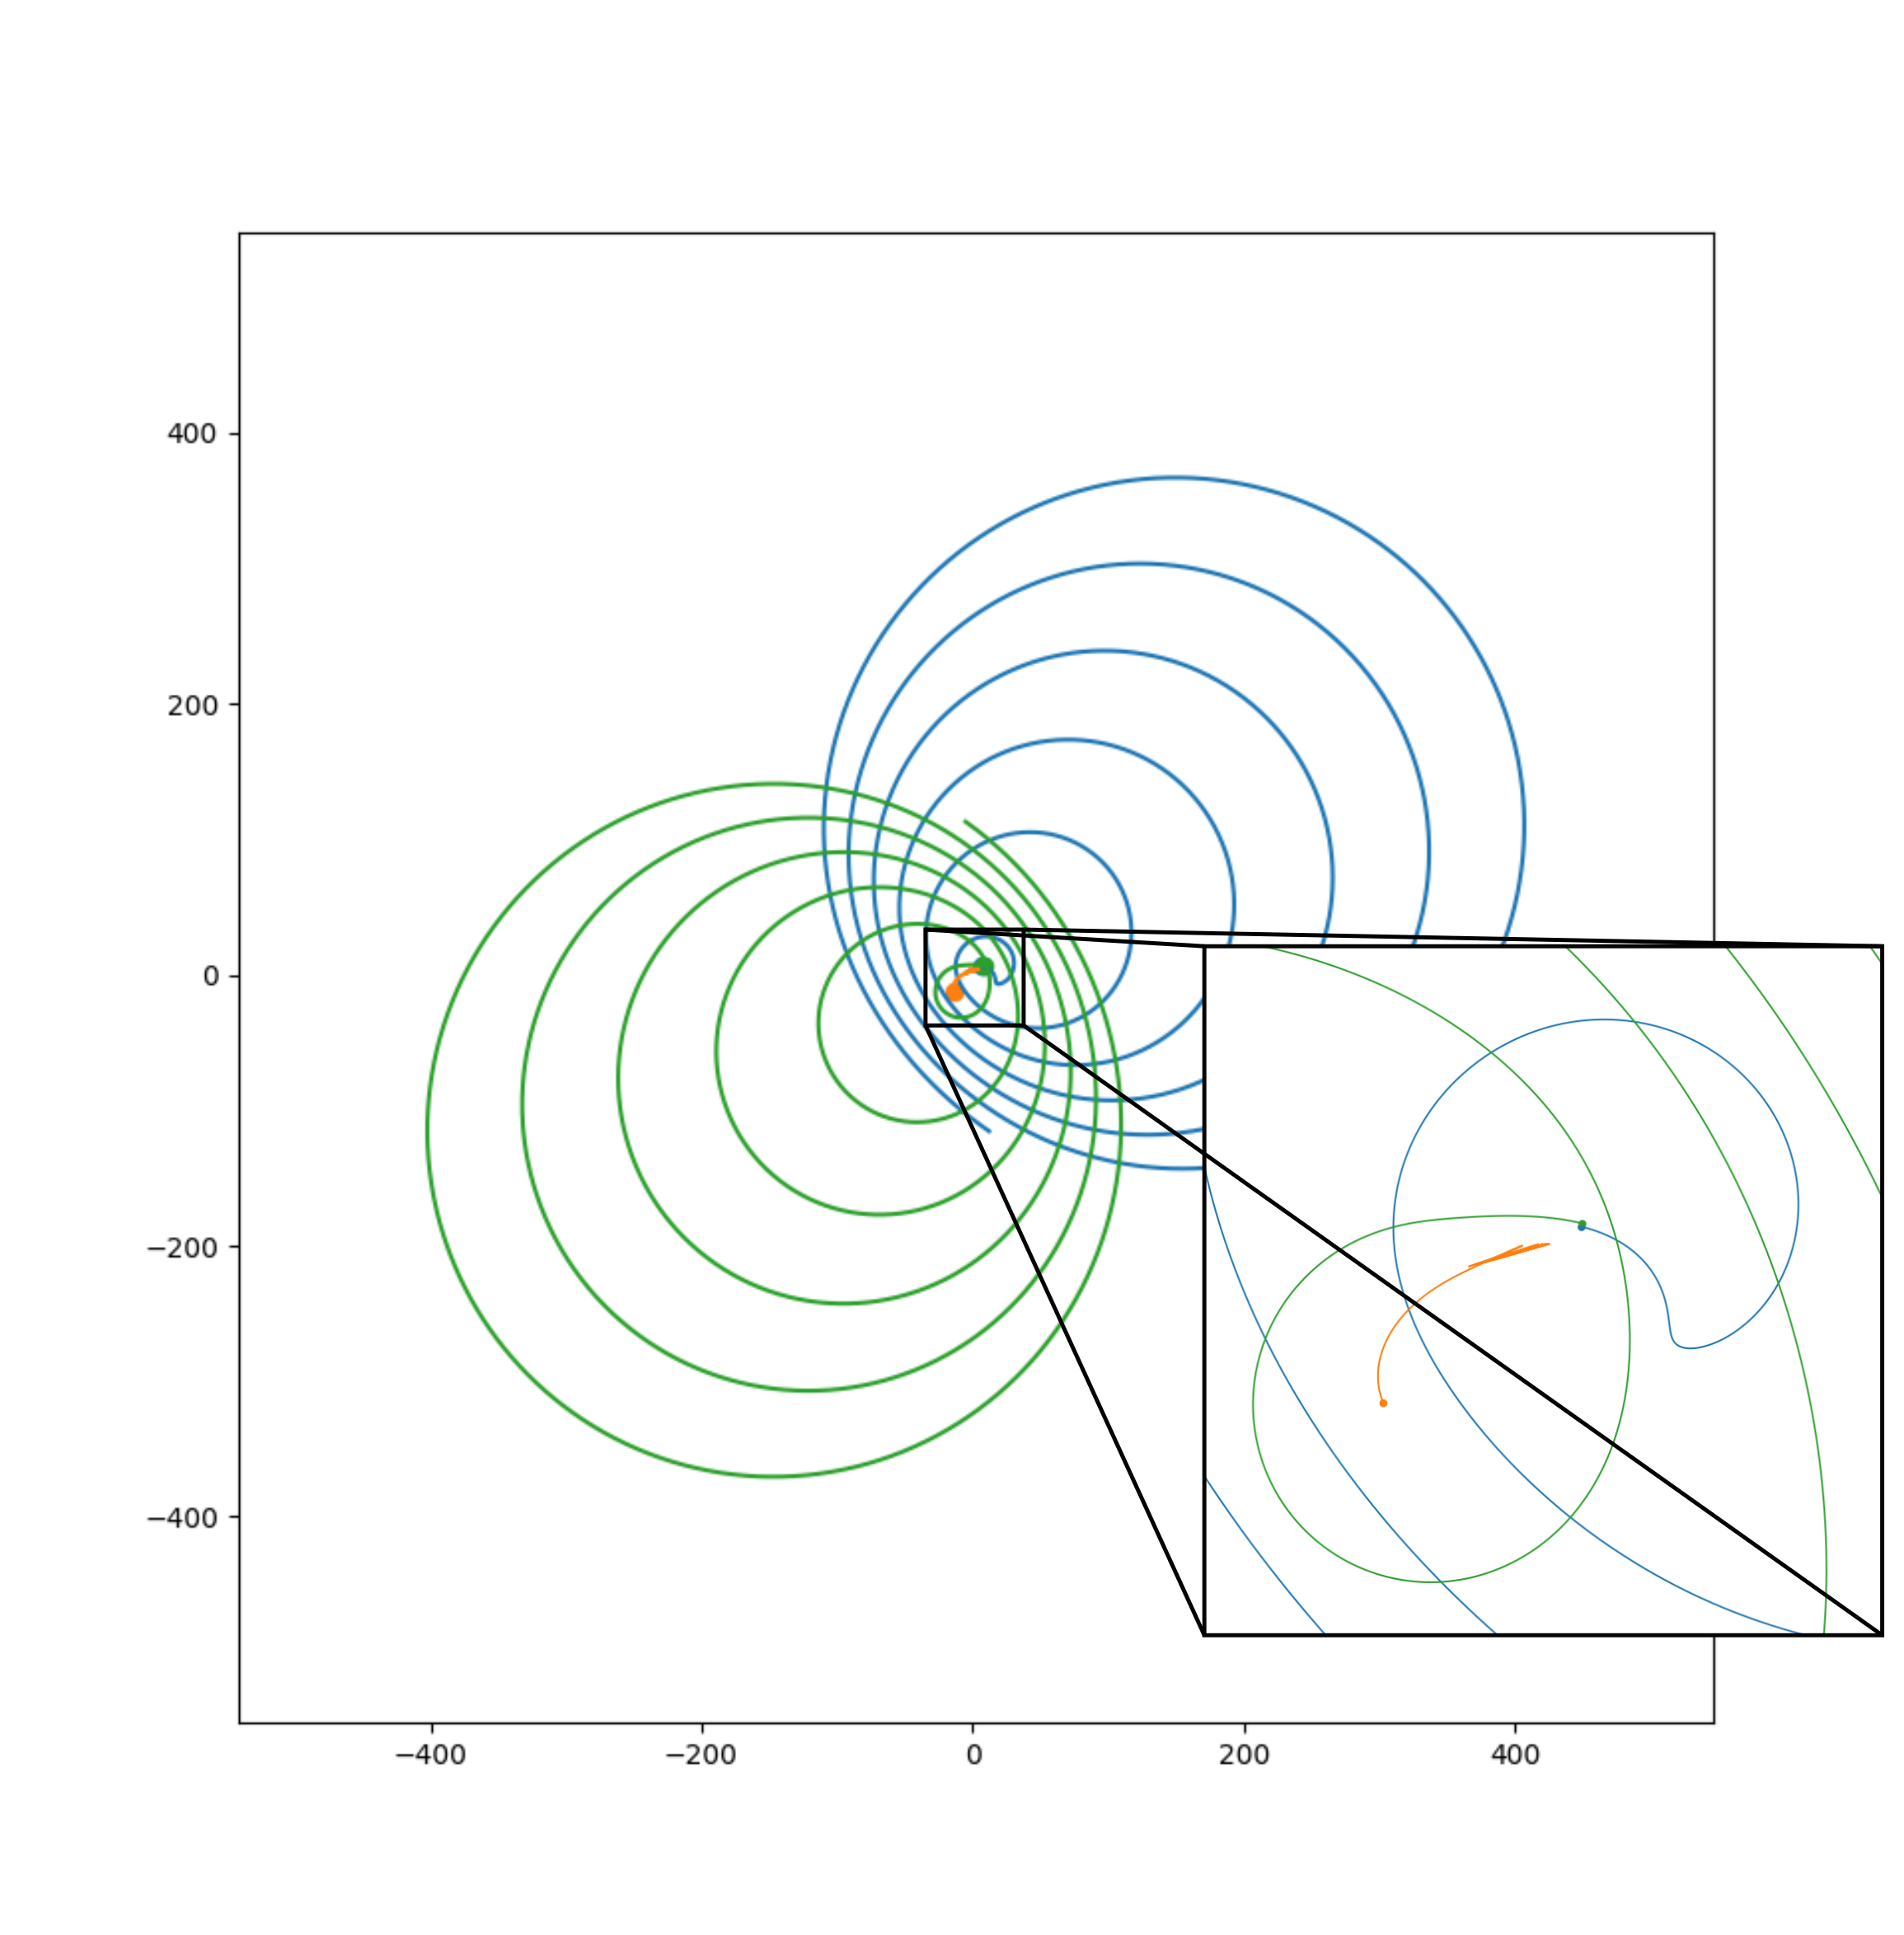
\includegraphics[width=\linewidth]{tcc//img/3corpos_energia0_velocidades_sd_zoom.png}
        \caption{Momentos de forma ($\vet \pi$).}
        \label{fig:3corpos_energia0_velocidades_sd}
    \end{subfigure}
    \caption{Coordenadas objetivas $(\vet \sigma, \vet \pi)$ do problema-modelo \ref{probmodelo:3corpos_energia_nula}.}
    \label{fig:probmodelo3corposenergia0_sd}
\end{figure}

Testamos também o comportamento de um sistema de 3 corpos com energia $E>0$, o problema-modelo \ref{probmodelo:3corpos_energia_positiva}, integrado no intervalo $[4.18,5000]$ via método SVCP8S15 com $h=10^{-4}$ sem correção. O motivo para o instante inicial específico é que o sistema começa com momento de dilatação negativo, e por facilidade foi fixado $h>0$, portanto no intervalo $[0,4.18)$ tem-se $D<0$, o que significa que o ponto de Janus para este caso está na vizinhança de $t=4.18$.

\begin{figure}[H]
    \centering
    \begin{subfigure}{.5\textwidth}
        \centering
        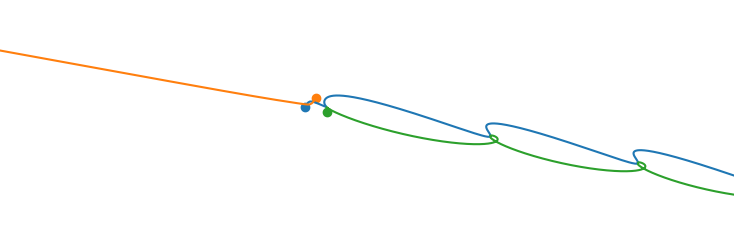
\includegraphics[width=0.8\linewidth]{tcc//img/3corpos_energiapositiva_posicoes_nd.png}
        \caption{}
        \label{fig:3corposenergiapositiva_trajetoria}
    \end{subfigure}%
    \begin{subfigure}{.5\textwidth}
        \centering
        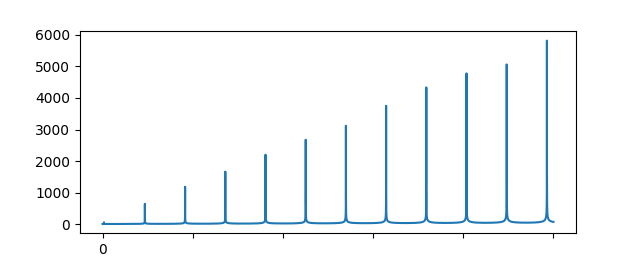
\includegraphics[width=\linewidth]{tcc//img/3corpos_energiapositiva_complexidade.png}
        \caption{}
        \label{fig:3corpos_energiapositiva_complexidade}
    \end{subfigure}
    
    \caption{Problema-modelo \ref{probmodelo:3corpos_energia_positiva}. À esquerda, recorte das trajetórias. À direita, a complexidade apresentada pelo sistema.}
    \label{fig:figuras_probmodel3_energia_positiva}
\end{figure}

Observe que neste problema os picos da complexidade são maiores (figura \ref{fig:3corpos_energiapositiva_complexidade}), refletindo a intensidade das aproximações do sistema binário formado. 

Isso se apresenta também nas coordenadas no espaço de formas. Como no problema com $E=0$, o corpo ejetado desacelera e começa a apresentar um comportamento cíclico e dissipativo (figura \ref{fig:3corpos_energiapositiva_posicoes_sd}). Porém, nesse caso a dissipação é bastante maior que no caso anterior. É visualmente notável a diferença na dissipação observando os momentos (figura \ref{fig:3corpos_energiapositiva_velocidades_sd}), pois o corpo dissipado tem momento oscilando próximo de zero e o sistema binário formado apresenta trajetórias circulares com raios cada vez maiores e com ordem de grandeza $10^5$, enquanto no caso $E=0$ tinha-se ordem de grandeza $10^2$.

\begin{figure}[H]
    \centering
    \begin{subfigure}{.5\textwidth}
        \centering
        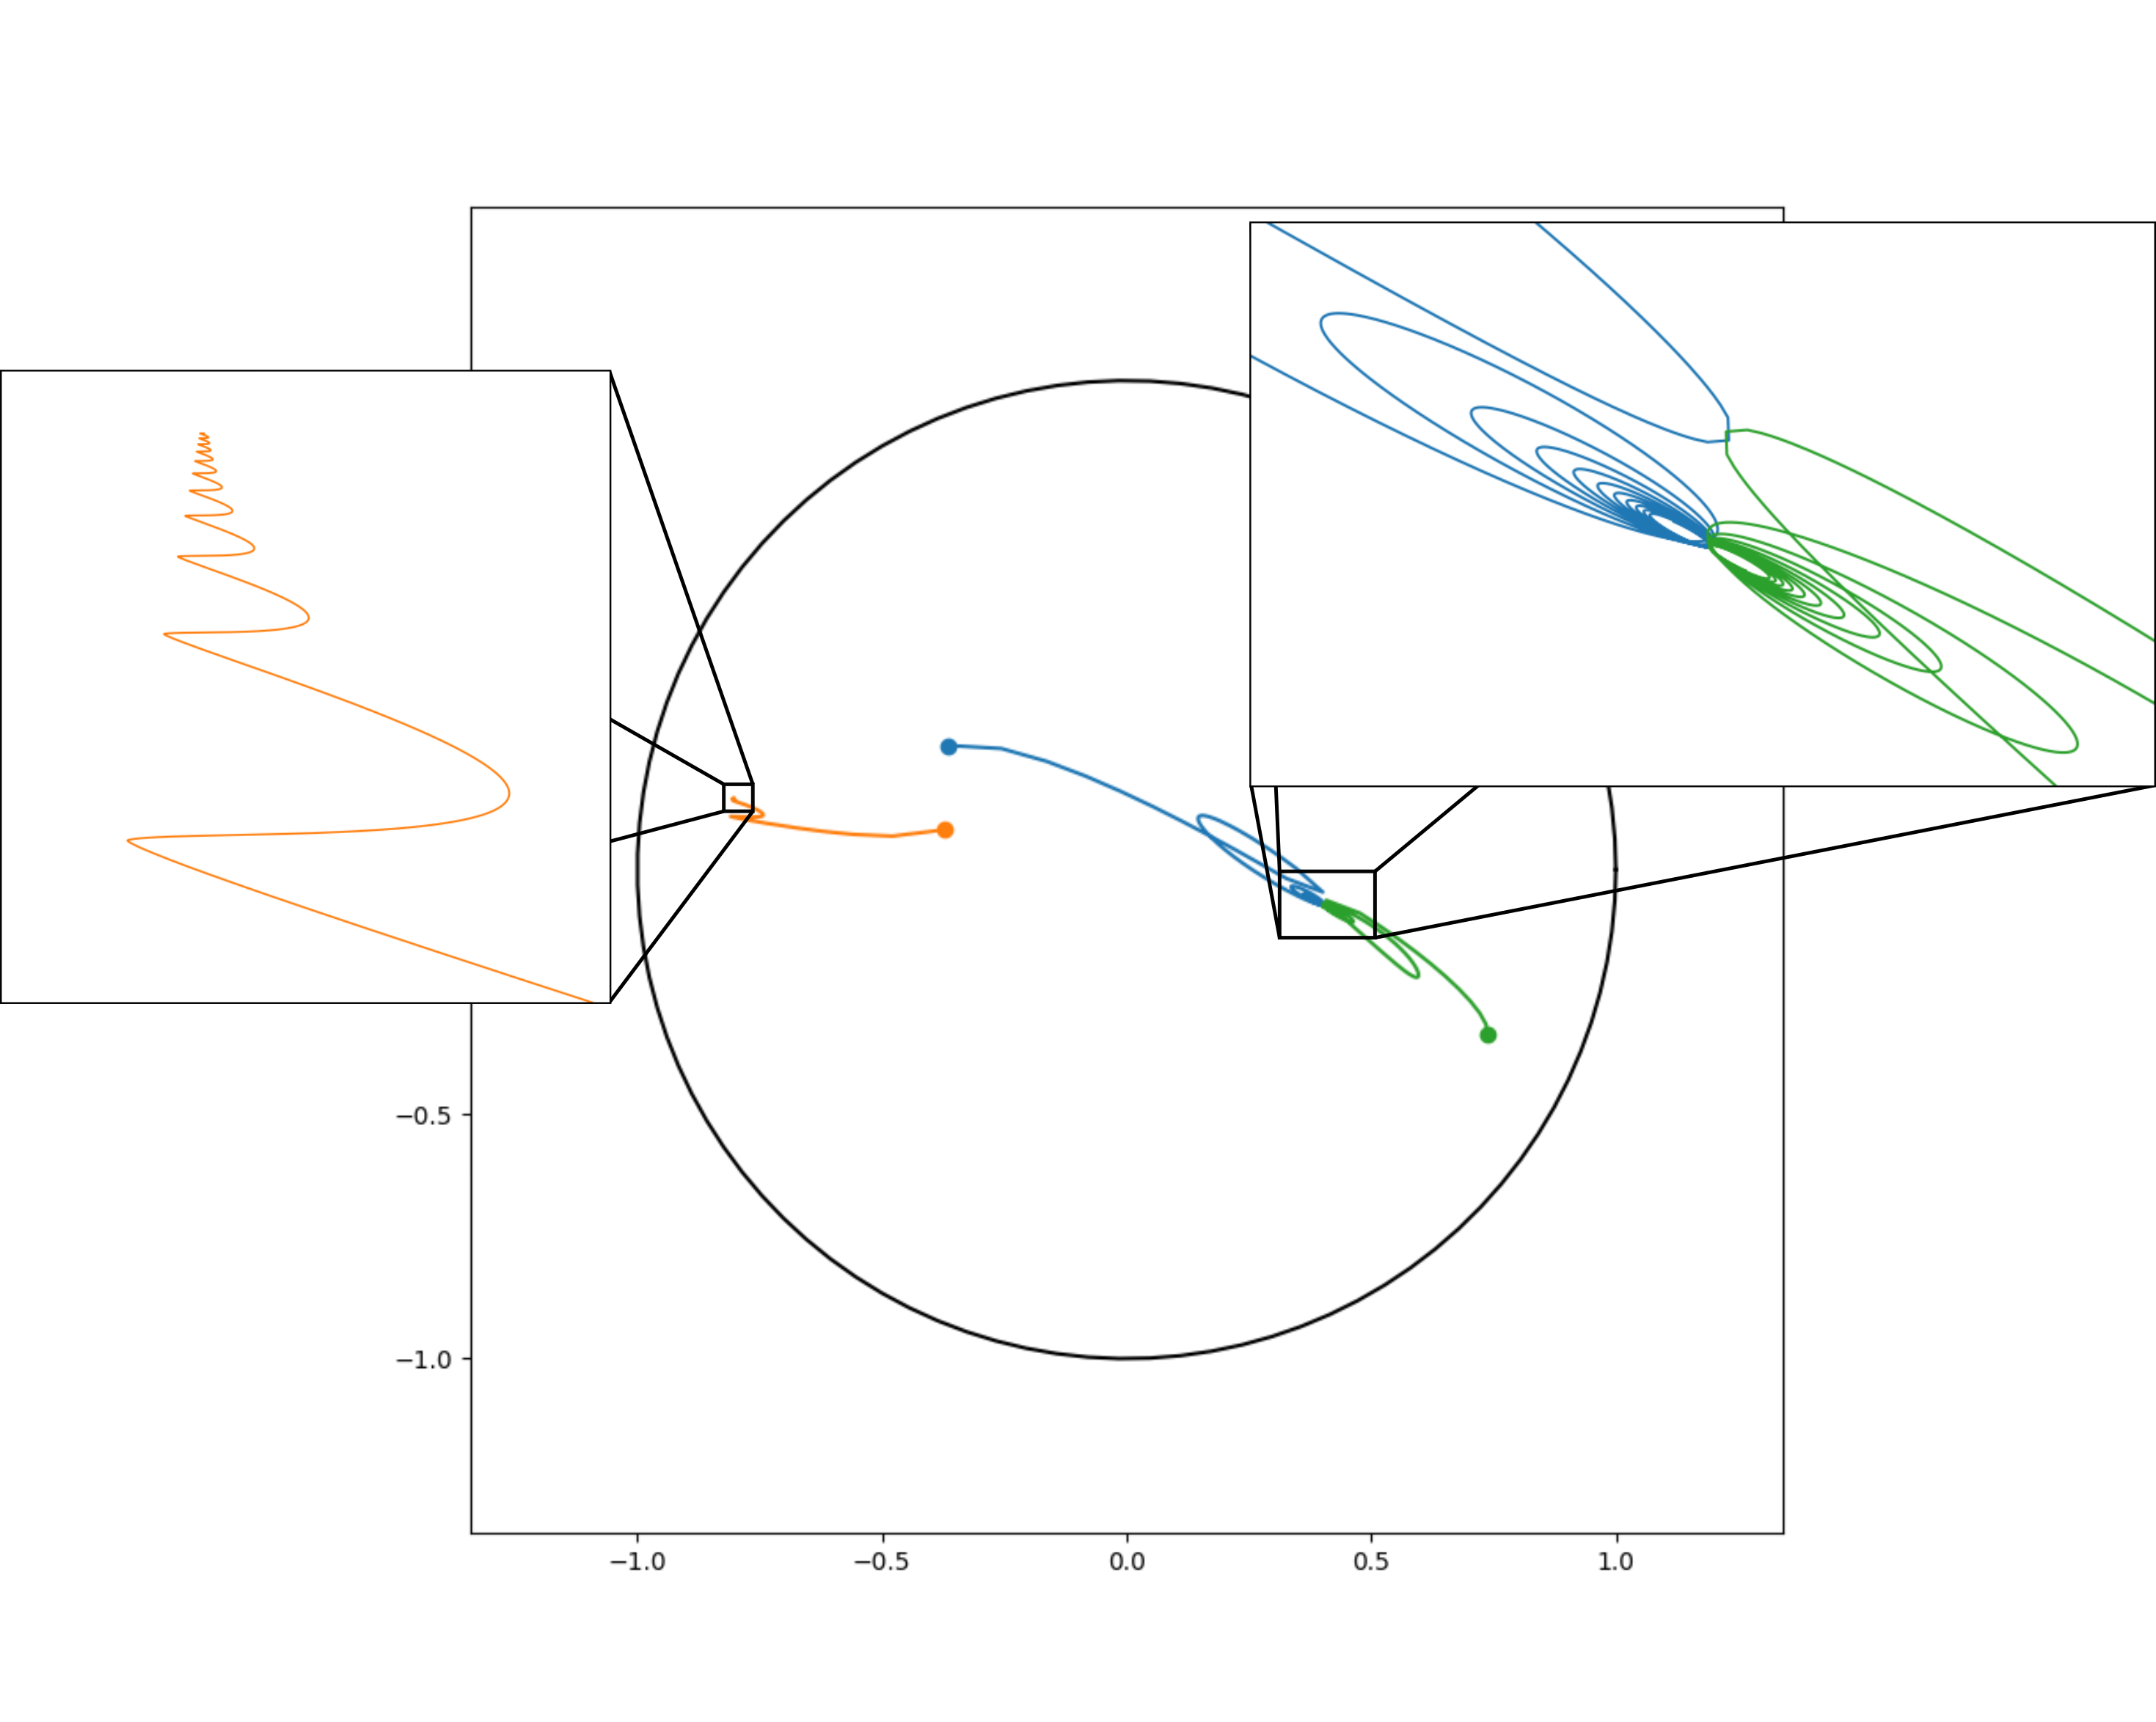
\includegraphics[width=\linewidth]{tcc//img/3corpos_energiapositiva_posicoes_sd_zoom.png}
        \caption{Coordenadas de forma ($\vet \sigma$).}
        \label{fig:3corpos_energiapositiva_posicoes_sd}
    \end{subfigure}%
    \begin{subfigure}{.5\textwidth}
        \centering
        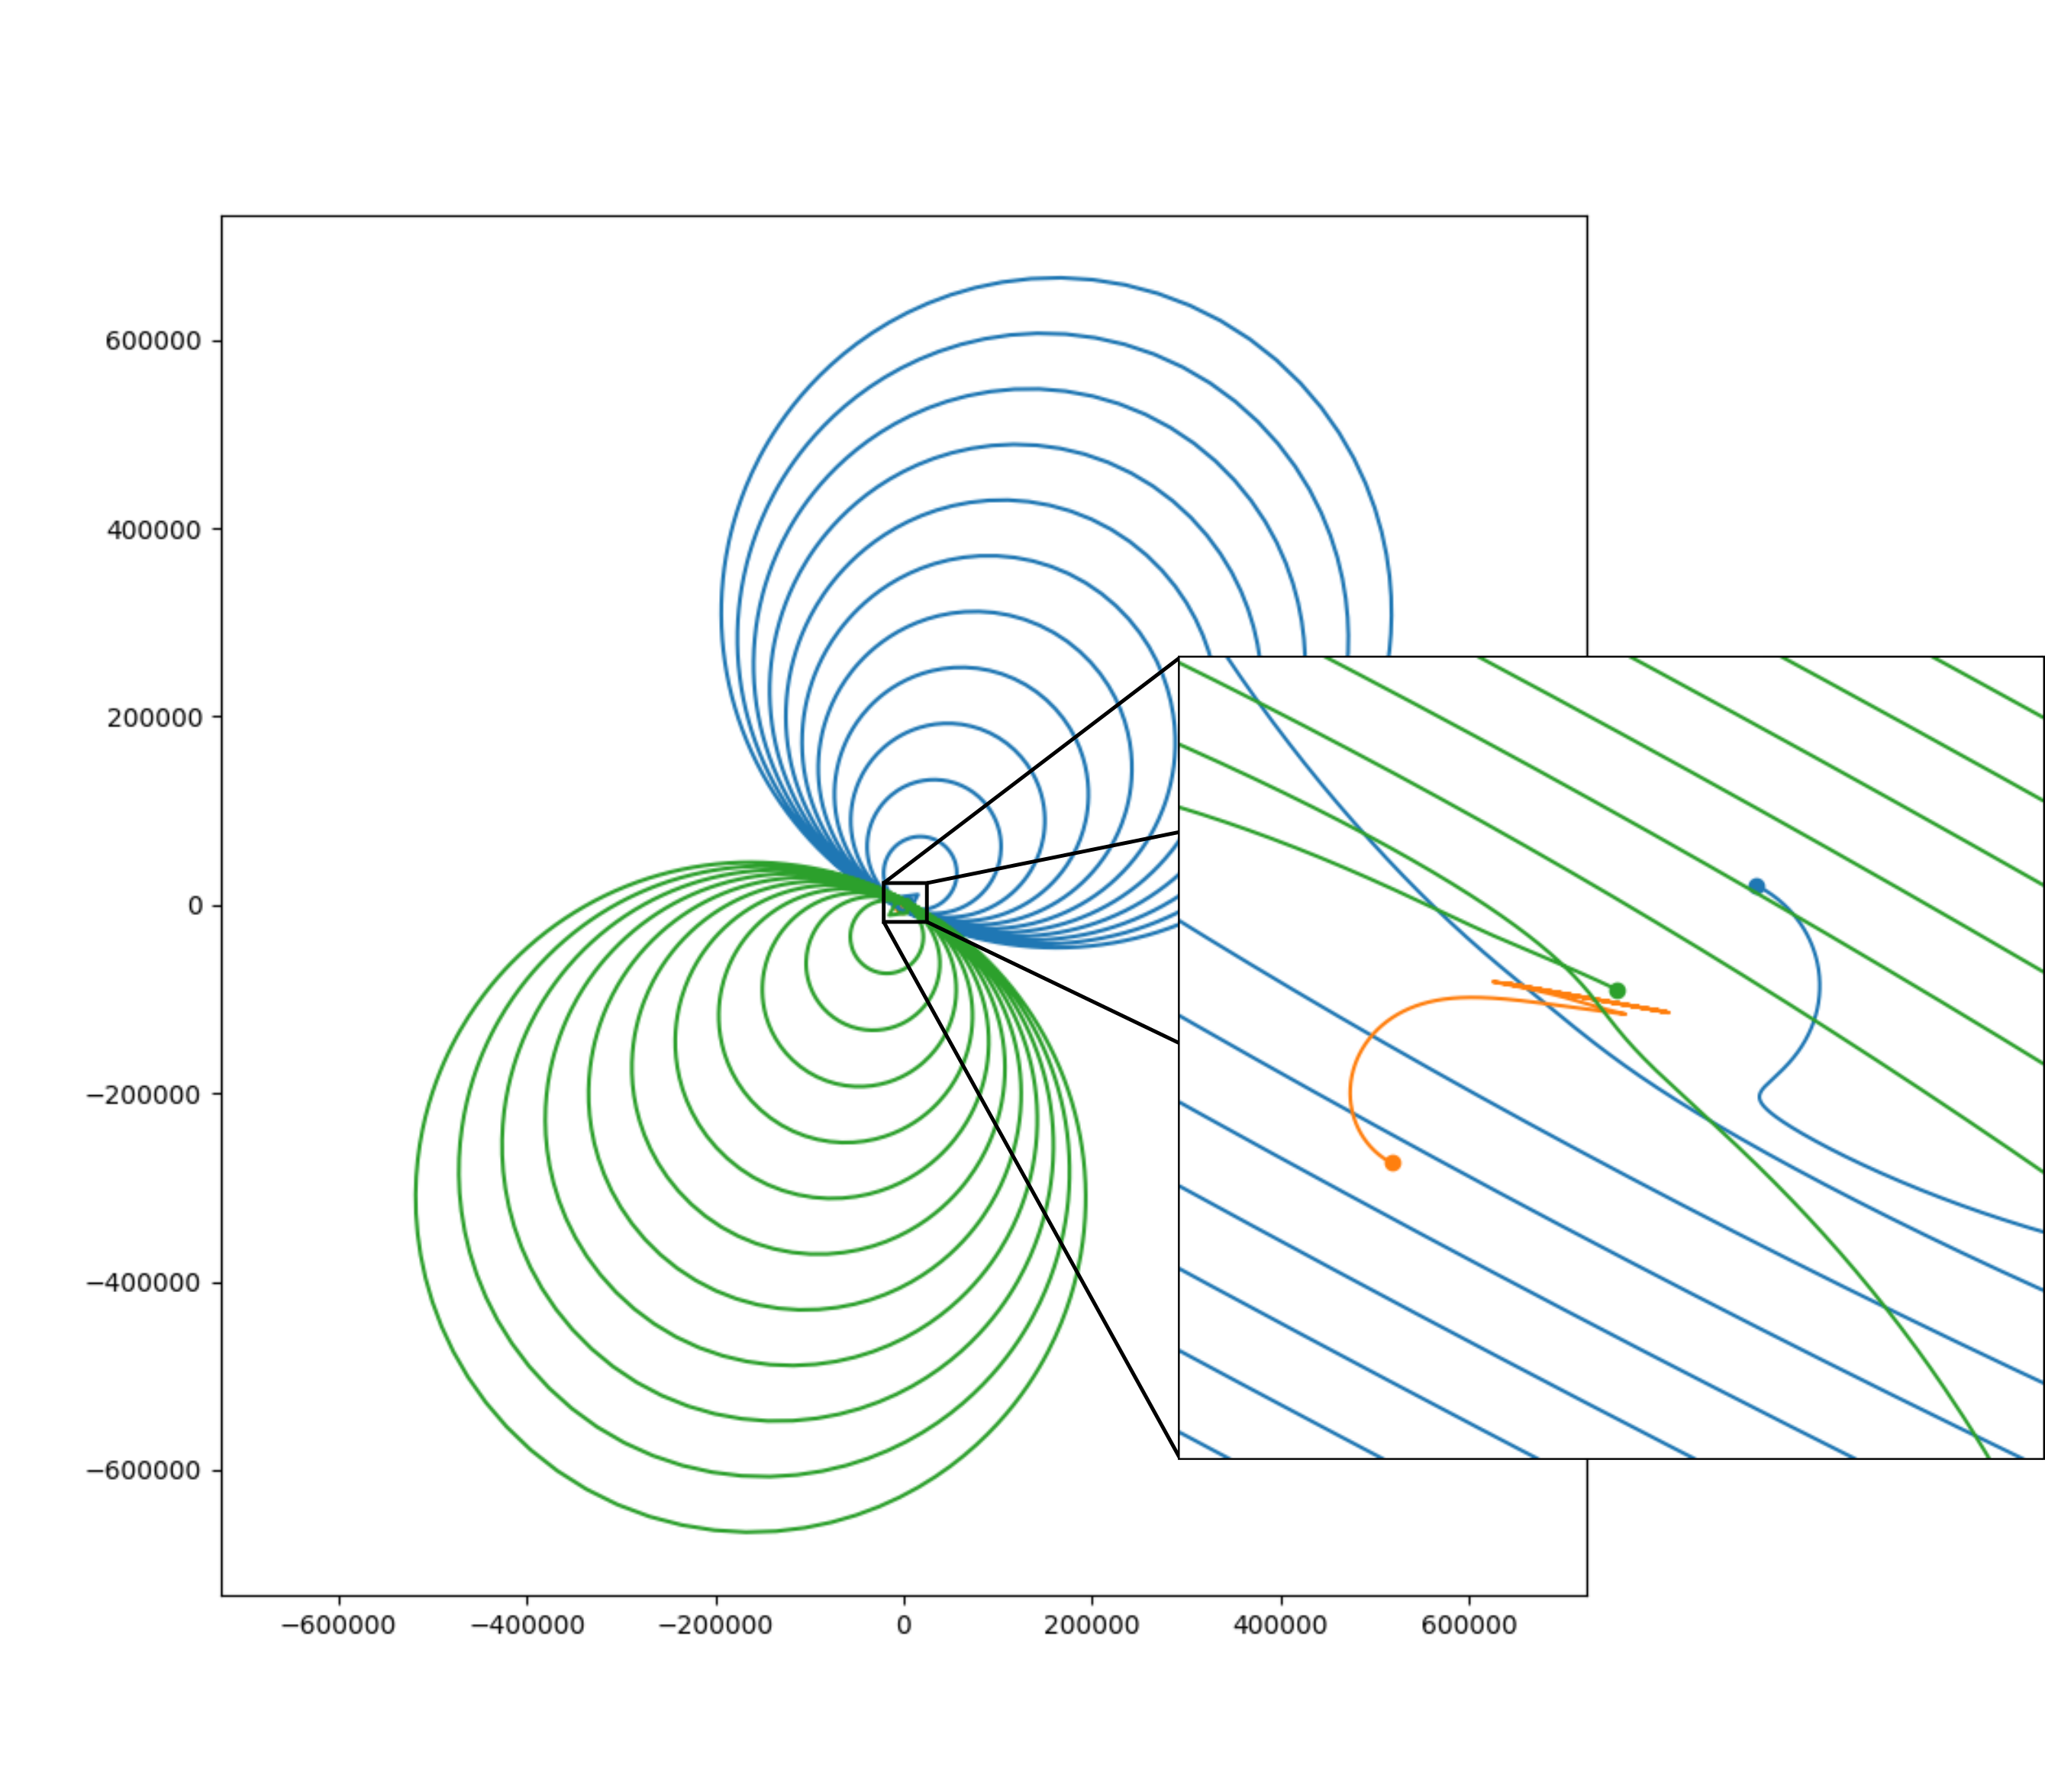
\includegraphics[width=\linewidth]{tcc//img/3corpos_energiapositiva_velocidades_sd_zoom.png}
        \caption{Momentos de forma ($\vet \pi$).}
        \label{fig:3corpos_energiapositiva_velocidades_sd}
    \end{subfigure}
    \caption{Coordenadas objetivas $(\vet \sigma, \vet \pi)$ do problema-modelo \ref{probmodelo:3corpos_energia_positiva}.}
    \label{fig:probmodelo3corposenergiapositiva_sd}
\end{figure}




%%%%%%%% PROBLEMA DE 20 CORPOS
\subsection{Problemas de 20 e 100 corpos}

Para problemas com $N \geq 10$, se mostrou pouco produtivo analisar as trajetórias no espaço de formas devido à quantidade de trajetórias. Além disso, dada a obrigatória separação do sistema em subsistemas em afastamento mútuo, a evolução no tempo newtoniano aumenta o momento de inércia $R^2$ mais rapidamente que o afastamento entre os corpos, levando as trajetórias no centro da esfera unitária a esferas cada vez menores e os corpos distantes a desacelerarem em algum ponto da esfera. 

\begin{figure}
    \centering
    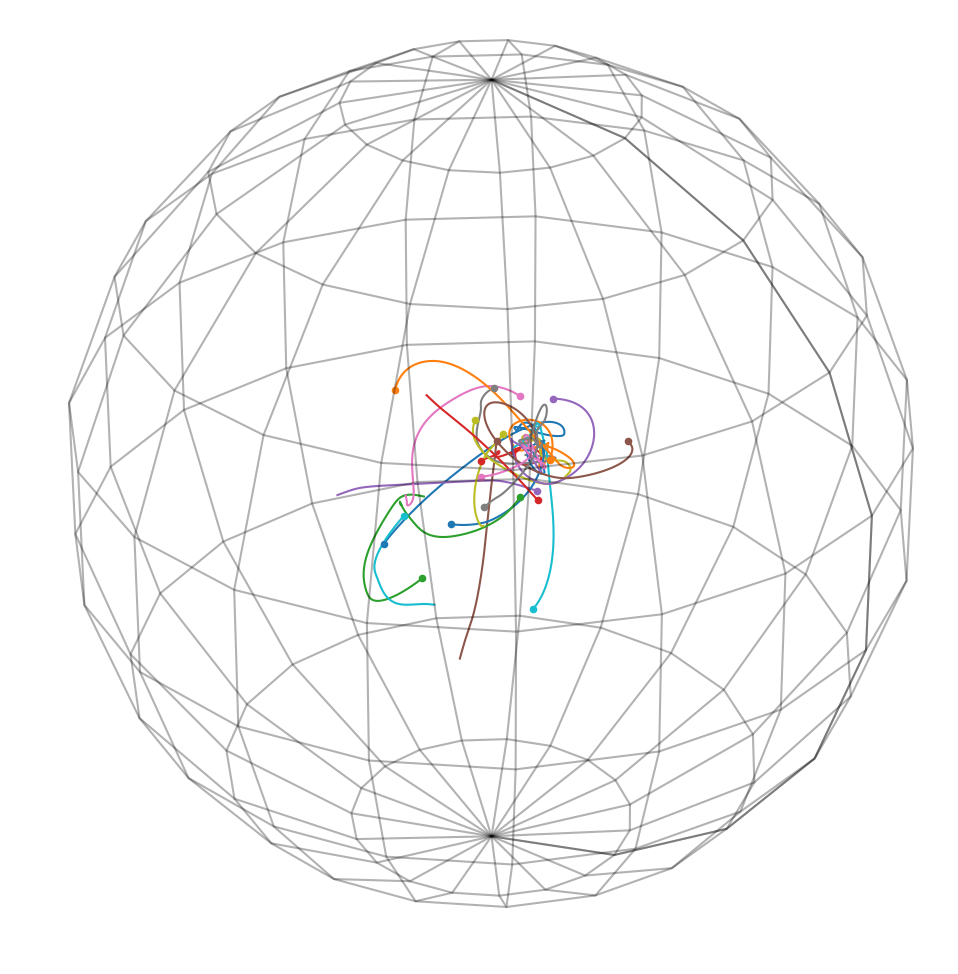
\includegraphics[width=0.5\linewidth]{tcc//img/20corpos_energia0_posicoes_3d_sd.png}
    \caption{Trajetória objetiva do problema-modelo \ref{probmodelo:20corpos_energia0}.}
    \label{fig:20corpos_trajetorias_sd}
\end{figure}

Para visualizar esse comportamento, simulamos o problema-modelo \ref{probmodelo:20corpos_energia0} com 20 corpos no intervalo $[0,5000]$ via RKN671 com $h=10^{-2}$ e $\epsilon=8h$. Nesse problema, todas as integrais primeiras são nulas. A trajetória objetiva pode ser visualizada na figura \ref{fig:20corpos_trajetorias_sd}.

A complexidade (figura \ref{fig:20corpos_complexidade}), porém, para $N=20$ já apresenta mais nitidamente o comportamento esperado: a expansão do sistema (grande escala) faz com que $C_S$ cresça no tempo newtoniano, e as interações entre os subsistemas (pequena escala) se apresentam nas variações desse crescimento, bastante nítidas nos casos de aproximações intensas facilmente identificáveis pelos maiores picos de $C_S$.

\begin{figure}[H]
    \centering
    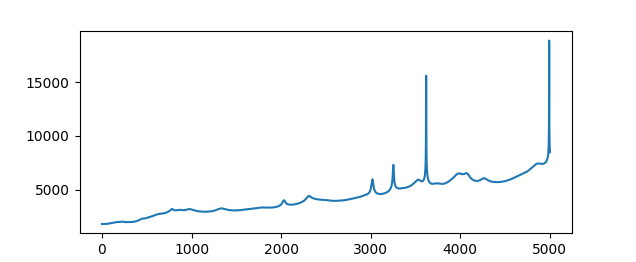
\includegraphics[width=0.8\linewidth]{tcc//img/20corpos_energia0_complexidade.png}
    \caption{Complexidade do problema-modelo \ref{probmodelo:20corpos_energia0}.}
    \label{fig:20corpos_complexidade}
\end{figure}

Simulamos também um problema de 100 corpos com todas as integrais primeiras nulas (\ref{probmodelo:100corpos_energia0}) no intervalo $[-10^6,10^6]$ via método de Verlet com $h=0.04=\epsilon$ em paralelo. Vale ressaltar que a simulação levou cerca de 108 segundos.

Na figura \ref{fig:100corpos_complexidade} podemos observar como as propriedades da complexidade se mostram ainda mais nítidas que no caso $N=20$. Além disso, como foi feita também a integração para o passado, é possível visualizar o ponto de Janus (o mínimo de $C_S$). Nesse caso, dada a grande variação de $C_S$, é possível observar que o sistema não apresentou grande expansão num primeiro momento, mas uma quantidade grande de interações no centro de massas.

\begin{figure}
    \centering
    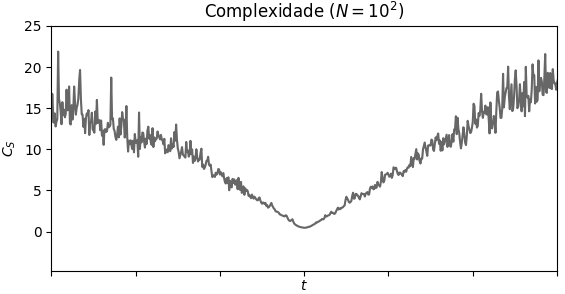
\includegraphics[width=0.6\linewidth]{tcc//img/complexidade100.png}
    \caption{Complexidade do problema-modelo \ref{probmodelo:100corpos_energia0}.}
    \label{fig:100corpos_complexidade}
\end{figure}


%%%%%%%% PROBLEMA DE 1000 CORPOS
\subsection{Problemas de 1000 corpos}

Passando para escalas maiores, realizamos três simulações com $N=10^3$ no intervalo $[-10^4, 10^4]$ via método de Verlet com $h=0.04=\epsilon=h$ para observar o comportamento de $C_S$ com diferentes valores de $E$: $-0.25$, $0$ e $0.25$.


\subsubsection{Energia total nula}

Começando pelos casos nos quais temos informações esperadas sobre o comportamento, o problema-modelo \ref{probmodelo:1000corpos_energianula} contém as condições iniciais para $E=0$ (todas as integrais primeiras são nulas, na verdade). Na figura \ref{fig:1000corpos_energia0_complexidade} é possível observar o crescimento variado de $C_S$ de maneira semelhante em relação ao eixo definido pelo Ponto de Janus. A vizinhança desse instante se apresentou nesse caso como um momento de rápida expansão e intensas aproximações, seguido pelo início de um momento de maior estabilidade tanto dos corpos ejetados quanto dos corpos ainda próximos ao centro. 

\begin{figure}[H]
    \centering
    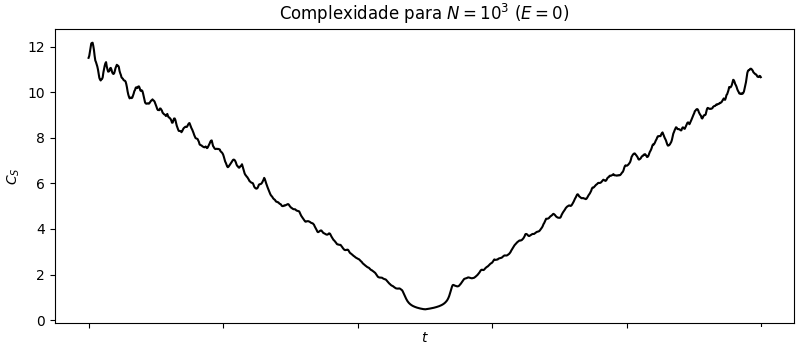
\includegraphics[width=0.6\linewidth]{tcc//img/complexidade_1000_nula.png}
    \caption{Complexidade do problema-modelo \ref{probmodelo:1000corpos_energianula}.}
    \label{fig:1000corpos_energia0_complexidade}
\end{figure}

A evolução do sistema pode ser observada na figura \ref{fig:1000corpos_energia0_posicoes}. O centro de massas concentra grande parte dos corpos mesmo nos limites do intervalo considerado, mas a ejeção de partículas continua acontecendo.

\begin{figure}[H]
    \centering
    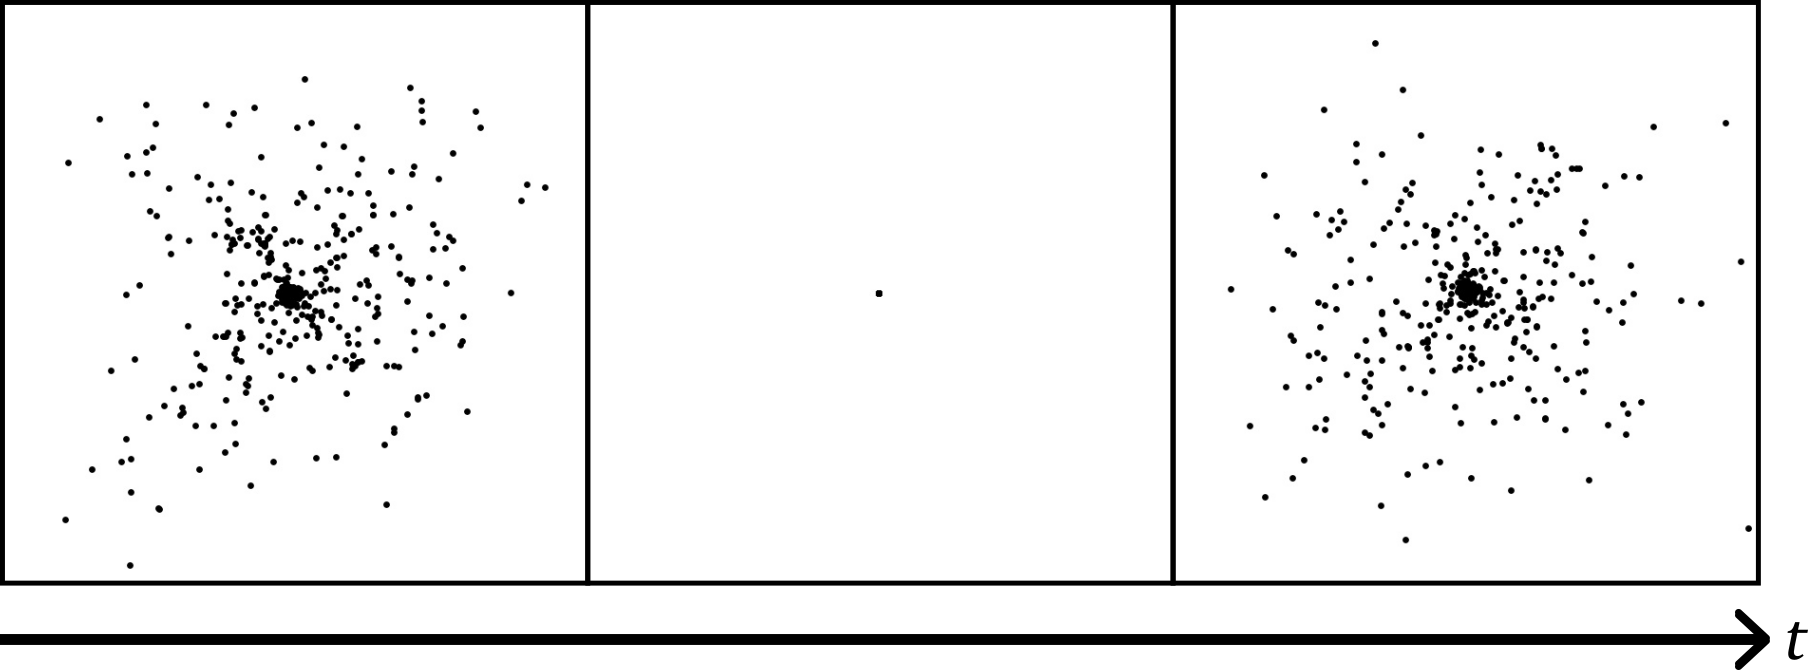
\includegraphics[width=0.8\linewidth]{tcc//img/espalhamento_energia_nula_1000.png}
    \caption{Instantes do bordo e $t=0$ do problema-modelo \ref{probmodelo:1000corpos_energianula}.}
    \label{fig:1000corpos_energia0_posicoes}
\end{figure}


\subsubsection{Energia total positiva}
Já para o caso $E=0.25$ no problema-modelo \ref{probmodelo:1000corpos_energiapositiva_1}, com massas $m=1/N$, observamos uma baixa variação de $C_S$ (figura \ref{fig:1000corpos_energiapositiva_complexidade_1}). Como o sistema necessariamente se contrai e se expande (devido ao comportamento do momento de inércia previsto pela relação de Lagrange-Jacobi), isso indica que a interação gravitacional entre os corpos é quase inversamente proporcional ao tamanho do sistema, o que sugere a não formação de binários e, do ponto de vista da do espaço de formas, o resultado é o esperado: o sistema assintoticamente congela.

\begin{figure}[H]
    \centering
    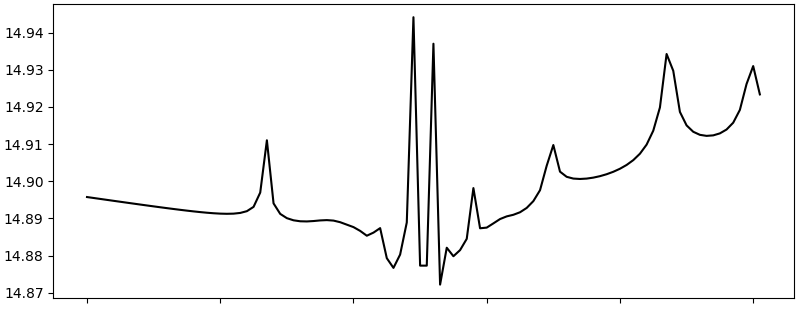
\includegraphics[width=0.6\linewidth]{tcc//img/1000corpos_energiapositiva_complexidade_1.png}
    \caption{Complexidade do problema-modelo \ref{probmodelo:1000corpos_energiapositiva_1}.}
    \label{fig:1000corpos_energiapositiva_complexidade_1}
\end{figure}

Na figura \ref{fig:1000corpos_energiapositiva_posicoes_1} é possível observar um espalhamento bastante uniforme dos corpos no espaço. Uma vez que os valores iniciais foram gerados através de uma distribuição uniforme, isso reflete o baixo nível de interação entre os corpos.

\begin{figure}[H]
    \centering
    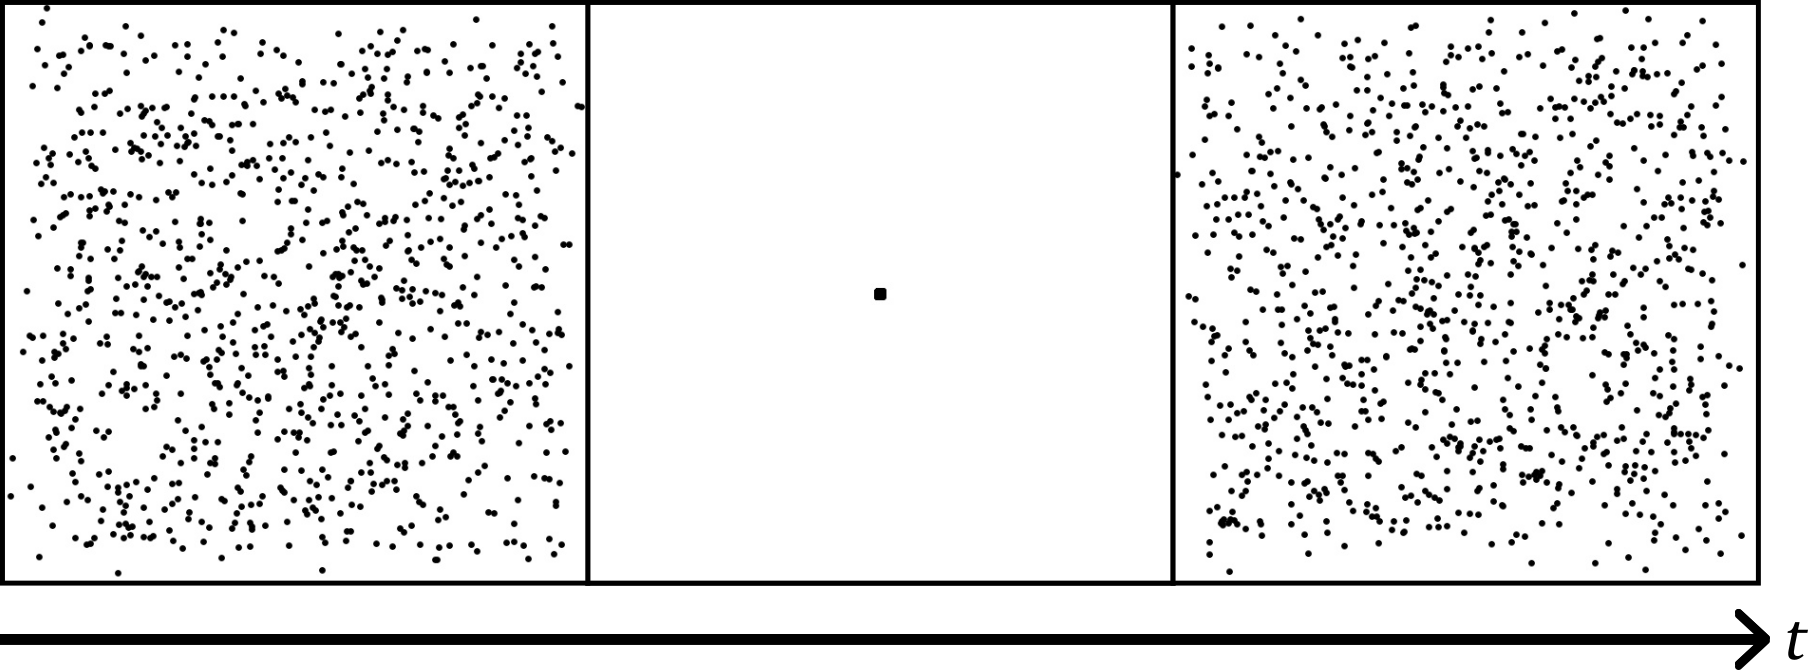
\includegraphics[width=0.8\linewidth]{tcc//img/espalhamento_energia_positiva_1000.png}
    \caption{Instantes do bordo e $t=0$ do problema-modelo \ref{probmodelo:1000corpos_energiapositiva_1}.}
    \label{fig:1000corpos_energiapositiva_posicoes_1}
\end{figure}


Optamos então por gerar novos valores iniciais mas com massas um pouco maiores individualmente, mas o suficiente para o sistema aumentar $10^3$ vezes em massa total (problema-modelo \ref{probmodelo:1000corpos_energiapositiva_2}). Nesse caso, o problema apresentou um comportamento mais parecido com o caso $E=0$, pois as interações gravitacionais foram mais intensas (veja figura \ref{fig:1000corpos_energiapositiva_posicoes_2}).

\begin{figure}[H]
    \centering
    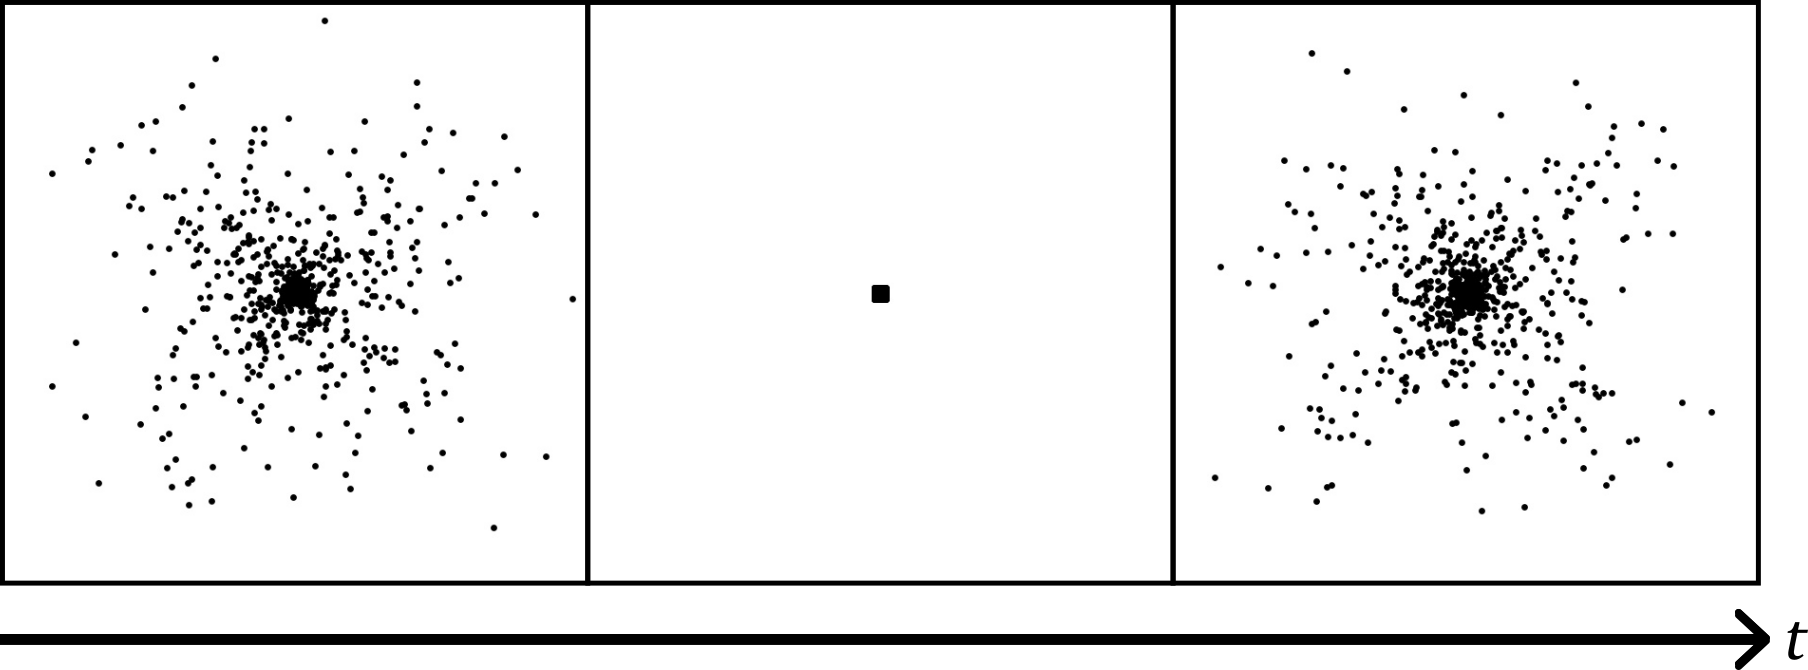
\includegraphics[width=0.8\linewidth]{tcc//img/espalhamento_energia_positiva_1000_2.png}
    \caption{Instantes do bordo e $t=0$ do problema-modelo \ref{probmodelo:1000corpos_energiapositiva_2}.}
    \label{fig:1000corpos_energiapositiva_posicoes_2}
\end{figure}

A complexidade também apresentou um comportamento diferente do primeiro exemplo de $E=0.25$ com um formato semelhante ao de $E=0$, mas com uma grande diferença de escala (veja figura \ref{fig:1000corpos_energiapositiva_complexidade_2}).

\begin{figure}
    \centering
    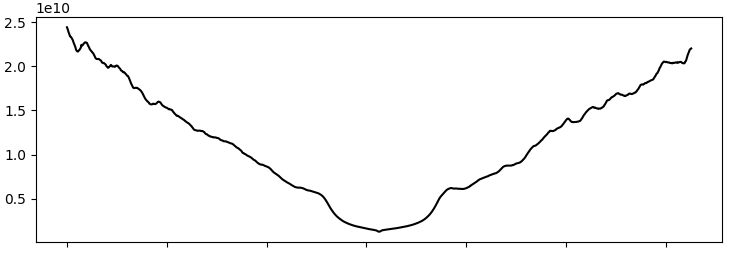
\includegraphics[width=0.8\linewidth]{tcc//img/1000corpos_energiapositiva_complexidade_2.png}
    \caption{Complexidade no problema-modelo \ref{probmodelo:1000corpos_energiapositiva_2}.}
    \label{fig:1000corpos_energiapositiva_complexidade_2}
\end{figure}


\subsubsection{Energia total negativa}
Por fim, no caso $E=-0.25$ tivemos um resultado curioso. Embora as condições impostas inicialmente tenham sido as de Hénon (veja subseção \ref{subsection:condicoes_aarseth}), a complexidade apresentou um comportamento de cúspide (figura \ref{fig:1000corpos_energianegativa_complexidade}. O que ocorre é que na evolução do sistema nesse caso são ejetados alguns corpos (o que provoca o crescimento) mas mantém relativa estabilidade no centro de massas.

\begin{figure}[H]
    \centering
    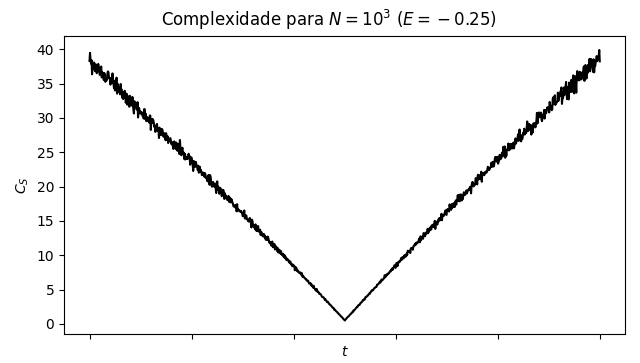
\includegraphics[width=0.6\linewidth]{tcc//img/complexidade1000_energianegativa.png}
    \caption{Complexidade no problema-modelo \ref{probmodelo:1000corpos_energianegativa}.}
    \label{fig:1000corpos_energianegativa_complexidade}
\end{figure}

Esse comportamento pode ser observado na figura \ref{fig:1000corpos_energianegativa_posicoes}, onde a maior parte do sistema fica contida na região central enquanto alguns poucos corpos são ejetados, sem formação de binários.

\begin{figure}[H]
    \centering
    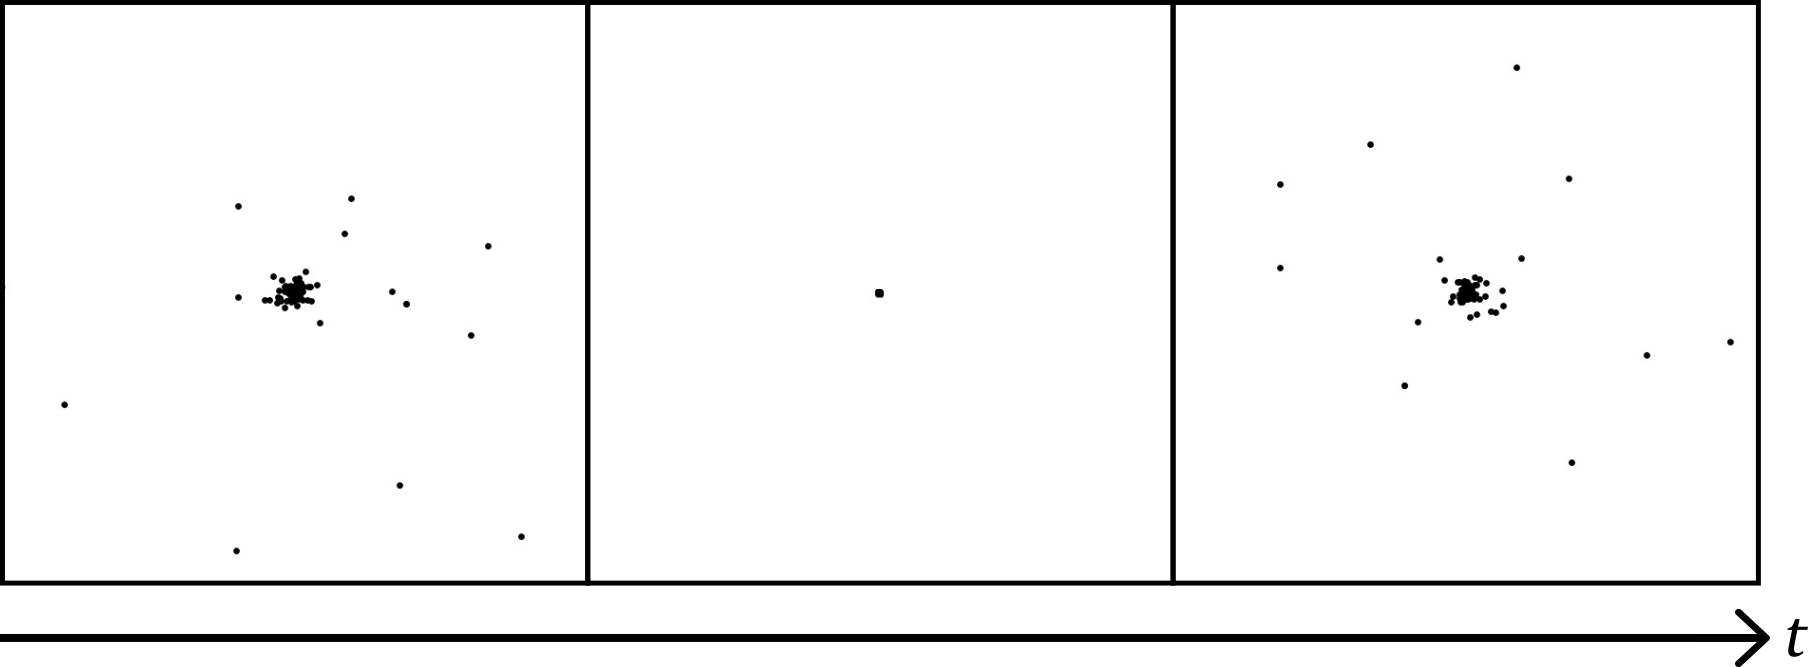
\includegraphics[width=0.8\linewidth]{tcc//img/espalhamento_energia_negativa_1000.png}
    \caption{Instantes do bordo e $t=0$ do problema-modelo \ref{probmodelo:1000corpos_energianegativa}.}
    \label{fig:1000corpos_energianegativa_posicoes}
\end{figure}

Na vizinhança do Ponto de Janus, porém, é possível encontrar semelhanças com os casos $E \geq 0$, como na formação de um pequeno ``vale'' a princípio seguido do início da variação (figura \ref{fig:1000corpos_energianegativa_complexidade_zoom}).

\begin{figure}[H]
    \centering
    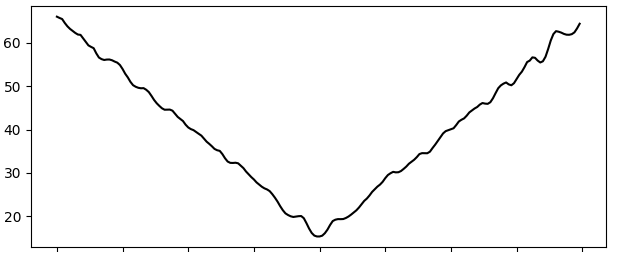
\includegraphics[width=0.8\linewidth]{tcc/img/zoom_complexidade_1000corpos_negativa.png}
    \caption{Vizinhança do ponto de Janus no problema $N=10^3$ com $E=-0.25$.}
    \label{fig:1000corpos_energianegativa_complexidade_zoom}
\end{figure}